\chapter{Υλοποίηση}

% TODO OPT: Note that we had set off to implement it from scratch but were
% working in parallel due to miscommunication?
Μία βασική υλοποίηση-σκελετός του \viofs{} προϋπήρχε στο \osv{}. % ref https://github.com/cloudius-systems/osv/commit/bae4381d1d0558b7a684294e9203864f9652395c
Αυτή υποστήριζε
απλή (μέσω της κλήσης \en{FUSE\_READ}) ανάγνωση αρχείων (και όχι καταλόγων).
Σε συνεννόηση με τα υπόλοιπα μέλη της κοινότητας του \osv{}, θέσαμε στόχο να
αναπτύξουμε περαιτέρω τη λειτουργικότητα αυτής της υλοποίησης. Το κομβικό
σημείο αυτής της προσπάθειας ήταν η υποστήριξη ανάγνωσης μέσω του \viofs{}
\en{DAX window}, κάτι που είχε σχεδιαστεί και υλοποιηθεί (σε ``πειραματικό''
ακόμα στάδιο) από τους ανθρώπους του \viofs{} με σκοπό την δραματική βελτίωση
των επιδόσεων του συστήματος αρχείων. Εκτός αυτού, είχαμε την ευκαιρία να
προσθέσουμε υποστήριξη για ανάγνωση καταλόγων, καθώς και εκκίνηση (\en{boot})
του \osv{} με το \viofs{} ως ριζικό (\en{root}) σύστημα αρχείων. Στην πορεία
απαιτήθηκαν δομικές αλλαγές, διορθώσεις και βελτιώσεις στην προϋπάρχουσα
υλοποίηση.

Σε αυτό το κεφάλαιο αναλύουμε την υλοποίηση των πιο ουσιαστικών από τις παραπάνω
συμβολές: της ανάγνωσης αρχείων μέσω \en{DAX window} και του \en{boot} από
\viofs{}.

\section{\en{DAX window} στο \viofs{}}

Το \osv{} ακολουθεί μία εσωτερική δομή συμβατή με αυτή των περισσότερων πυρήνων
γενικού σκοπού, ορίζοντας χωριστά τις έννοιες του οδηγού (\en{driver}) και του
συστήματος αρχείων. Οι οδηγοί (στο \en{drivers/}) είναι υπεύθυνοι για
την παροχή μίας διεπαφής (\en{interface}) κοινής για κάθε οικογένεια συσκευών
(αποθήκευσης \en{block}, δικτύου κλπ), η οποία επιτρέπει τη χρήση της εκάστοτε
συσκευής από τα υπόλοιπα υποσυστήματα του πυρήνα. Τα συστήματα αρχείων (στο
\en{fs/}) αποτελούν επίσης υλοποιήσεις μίας κοινής διεπαφής η οποία ορίζεται από
το εικονικό σύστημα αρχείων (\en{virtual file system}) του \osv{}. Αυτή η
διεπαφή αποτελείται από λειτουργίες όπως το άνοιγμα, το κλείσιμο, η ανάγνωση από
αρχείο, και άλλες. Τα συστήματα αρχείων συνήθως είναι υλοποιημένα πάνω από μία
συσκευή \en{block} και χρησιμοποιούν τη διεπαφή που αυτή παρέχει για να
``μεταφράσουν'' ανάμεσα στις υψηλού επιπέδου λειτουργίες του συστήματος αρχείων
και τις χαμηλού επιπέδου λειτουργίες της συσκευής αποθήκευσης. Υπάρχουν βεβαίως
εξαιρέσεις όπως το \en{NFS}, το οποίο υποστηρίζεται από το δικτυακό υποσύστημα.

Το \viofs{} είναι ιδιαίτερο στο γεγονός ότι, ως σύστημα αρχείων εξαρτάται από
την ομώνυμη συσκευή, η οποία δεν μπορεί να αντιμετωπιστεί ως μέλος κάποιας από
τις συνήθεις οικογένειες (πχ \en{block} ή δικτύου). Αυτό το χαρακτηριστικό το
κληρονομεί βεβαίως από το \en{FUSE}. Έτσι, αναπόφευκτα υπάρχει ισχυρή, ρητή
εξάρτηση του \viofs{} συστήματος αρχείων από τον οδηγό της \viofs{} συσκευής
(σχήμα \ref{fig:virtiofs-vs-others}), κάτι που βλέπουμε και στην περίπτωση του
\linux{}, όπου αυτά τα δύο είναι υλοποιημένα μαζί (στο
\en{fs/fuse/virtio\_fs.c}). Από τα παραπάνω γίνεται σαφές ότι η διάκριση
ανάμεσα σε \viofs{} οδηγό και σύστημα αρχείων (δηλαδή ο αντίστοιχος καταμερισμός
των λειτουργιών) είναι εύκαμπτη. Παρ' όλα αυτά, η παρουσίαση την υλοποίησης που
ακολουθεί γίνεται  υπό το πρίσμα αυτής της διάκρισης.

\begin{figure}
    \centering
    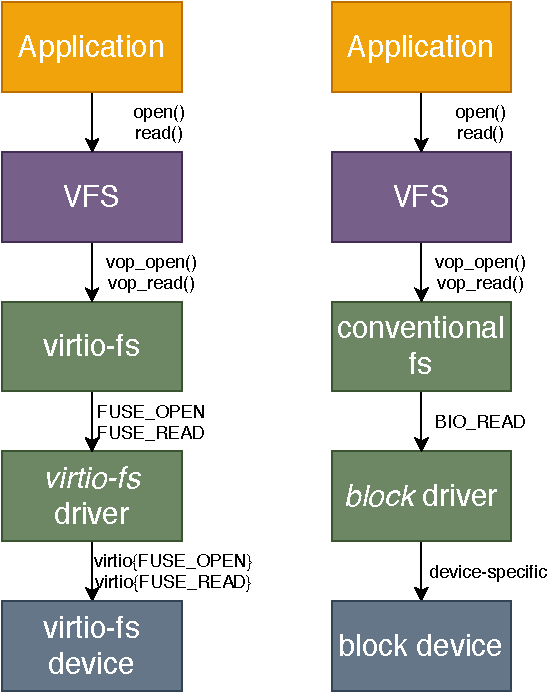
\includegraphics{virtiofs-vs-others}
    \caption{Συστατικά και εξαρτήσεις στον \guest{}: \viofs{} σε σύγκριση με
        συμβατικά συστήματα τοπικά αρχείων.}
    \label{fig:virtiofs-vs-others}
\end{figure}

\subsection{Οδηγός}

Ο οδηγός της \viofs{} συσκευής είναι επιφορτισμένος με την απευθείας επικοινωνία
με αυτή και τη χαμηλού επιπέδου διαχείριση της. Πέρα από την αρχικοποίηση
(ανακάλυψη \en{virtqueues}, διαπραγμάτευση παραμέτρων λειτουργίας)
\cite{virtio}, το κύριο έργο του είναι η μεταφορά αιτημάτων (\en{requests}) και
απαντήσεων (\en{responses}) σε αυτά από και προς τη συσκευή μέσω των
\en{virtqueues}. Γι' αυτό το σκοπό παρέχει μία ασύγχρονη διεπαφή υποβολής
αιτημάτων, στα οποία ενθυλακώνονται τα \en{FUSE} αιτήματα. Ο οδηγός παραμένει
αγνωστικός ως προς το \en{FUSE}, χειριζόμενος τα αιτήματα του ως αδιαφανή.

Η αρχικά διαθέσιμη υλοποίηση του \viofs{} \en{DAX window} στο \qemu{} ήταν ως
συσκευή \en{PCI}. Σύμφωνα με την προδιαγραφή του \en{virtio} \cite{virtio}
για τη συσκευή, το \en{DAX window} είναι η περιοχή κοινής μνήμης (\en{shared
memory region}) με αναγνωριστικό (``\en{shmid}'') 0. Στην περίπτωση του
\en{virtio PCI transport}, οι περιοχές κοινής μνήμης υλοποιούνται ως
\en{PCI BARs (base address registers)}, κάθε ένα εκ των οποίων εκτίθεται ως ένα
\en{VIRTIO\_PCI\_CAP\_SHARED\_MEMORY\_CFG PCI capability}, έχοντας ένα μοναδικό
αναγνωριστικό \cite{virtio, wiki:pci-conf, osdev:pci}.

Το πρώτο βήμα για την προσθήκη του \en{DAX window} ήταν λοιπόν η ανακάλυψη
(\en{discovery}) αυτού, εφόσον παρέχονταν από τη συσκευή. Αυτή ήταν μία ανώδυνη
εργασία, χάρη στο πλήρες και καλά μοντελοποιημένο υποσύστημα \en{PCI} του
\osv{}. Συγκεκριμένα, οι επιμέρους αλλαγές που χρειάστηκαν ήταν:
\begin{enumerate}
    \item Προσθήκη στο \en{PCI} υποσύστημα ώστε να είναι δυνατή η ανακάλυψη
          πολλαπλών \en{capabilities} με τον ίδιο τύπο (στο
          \en{drivers/pci-function.cc}). Αυτή ήταν απαραίτητη διότι μέχρι
          πρότινος οι λειτουργίες ανακάλυψης στο \osv{} αναζητούσαν μέχρι και το
          πρώτο \en{capability} ενός τύπου, σταματώντας εκεί. Όμως, όπως
          αναφέραμε προηγουμένως, κάθε περιοχή κοινής μνήμης αντιστοιχεί σε ένα
          \en{PCI capability} και αυτές μπορεί να είναι περισσότερες από μία (αν
          και στην περίπτωση του \viofs{} υπάρχει μόνο μία).
    \item Επέκταση στο μοντέλο των \en{virtio PCI} συσκευών (στο    % TODO OPT: Rephrase to avoid overfull hbox
          \en{drivers/virtio-pci-device.cc}) ώστε να ανακαλύπτει όλες τις
          περιοχές κοινής μνήμης κάθε συσκευής, αναζητώντας τα \en{capabilities}
          αντίστοιχου τύπου και αποθηκεύοντας τα στοιχεία (διεύθυνση και
          μέγεθος) των \en{BARs} που αυτά υποδεικνύουν.
    \item Επέκταση στον οδηγό της \viofs{} συσκευής (στο
          \en{drivers/virtio-fs.cc}) ώστε να ανακαλύπτει την περιοχή κοινής
          μνήμης με αναγνωριστικό 0, δηλαδή το \en{DAX window} και να το εκθέτει
          απευθείας στη διεπαφή του, ως περιοχή \en{MMIO (memory-mapped I/O)}
          της συσκευής. Σημειώνεται ότι η απεικόνιση (\en{mapping}) της περιοχής
          στον εικονικό χώρο διευθύνσεων έχει ήδη πραγματοποιηθεί από το μοντέλο
          της συσκευής.
\end{enumerate}

\subsection{Σύστημα αρχείων}

Το \viofs{} σύστημα αρχείων θεωρεί δεδομένο έναν μηχανισμό αποστολής \en{FUSE}
αιτημάτων (ο οποίος παρέχεται από τον οδηγό) και πάνω σε αυτόν χτίζει τη
λειτουργικότητα του. Είναι συνεπώς επιφορτισμένο με τη γνώση και τον
χειρισμό του περιεχομένου των αιτημάτων που ο οδηγός απλώς μεταφέρει.

\subsubsection{Απεικόνιση αρχείων}

Η προσάρτηση (\en{mounting}) ενός \viofs{} συστήματος αρχείων συνίσταται στην
έναρξη μίας \en{FUSE} συνεδρίας (\en{session}) με την αποστολή ενός
\en{FUSE\_INIT} αιτήματος \cite{virtio}. Με αυτό πραγματοποιείται η
διαπραγμάτευση των παραμέτρων της συνεδρίας, μεταξύ των οποίων και μίας που
αφορά τη λειτουργία του \en{DAX window}: η ευθυγράμμιση των απεικονίσεων
(\en{map alignment}). Η πρώτη τροποποίηση που απαιτούνταν στο σύστημα αρχείων
λοιπόν ήταν η επέκταση της διαδικασίας προσάρτησης ώστε να γνωστοποιείται στη
συσκευή ότι υποστηρίζεται από το λειτουργικό το \en{DAX window} και να
λαμβάνεται η τιμή της παραμέτρου από την απάντηση.

Η παραπάνω παράμετρος περιορίζει τα \en{mappings} αρχείων στο \en{DAX window} ως
εξής: τόσο η μετατόπιση (\en{offset}) της αρχής ενός \en{mapping} μέσα στο
αρχείο όσο και στο \en{DAX window} πρέπει να είναι ευθυγραμμισμένες σύμφωνα με
το \en{map alignment}. Αυτό στην πράξη επιβάλλεται στην παρούσα υλοποίηση της
\viofs{} συσκευής από τη χρήση της \texttt{\en{mmap()}} \cite{man:mmap} στον
\host{} (επίσης ο λόγος που το \en{map alignment} συνήθως ταυτίζεται με το
μέγεθος της σελίδας μνήμης στον \host{}).

Όπως ορίζεται από την προδιαγραφή, η παροχή του \en{DAX window} από τη συσκευή
όπως και η χρησιμοποίηση του από τον \guest{} είναι αμφότερα προαιρετικά.
Επίσης, η χρήση του \en{DAX window} είναι ανεξάρτητη από τη χρήση της συμβατικής
\en{FUSE\_READ} (που είναι πάντοτε διαθέσιμη) για την ανάγνωση αρχείων. Έτσι, η
υλοποίηση μας, εφόσον είναι διαθέσιμο το \en{DAX window}, επιχειρεί να
ικανοποιήσει όλες τις αναγνώσεις αρχείων μέσω εκείνου. Σε περίπτωση όμως που
αυτό δεν είναι διαθέσιμο ή αποτύχει η διαδικασία της ανάγνωσης από εκείνο,
στρέφεται δυναμικά στην εφεδρική \en{FUSE\_READ}, όπως φαίνεται και στο
διάγραμμα \ref{fig:dax-flowchart}.

\begin{otherlanguage}{english}
\begin{lstlisting}[
    float,
    caption=\gr{Ορισμοί του \en{FUSE} για τις λειτουργίες απεικονίσεων. Βλέπε
        παράρτημα \ref{app:copyright} για σημείωμα πνευματικών δικαιωμάτων.},
    label=lst:fuse-defs,
    language=C,
    captionpos=b,
    frame=single,
    basicstyle=\ttfamily,
    commentstyle=\color{olive},
    keywordstyle=\color{blue}]
#define FUSE_SETUPMAPPING_FLAG_WRITE (1ull << 0)
struct fuse_setupmapping_in {
    /* An already open handle */
    uint64_t        fh;
    /* Offset into the file to start the mapping */
    uint64_t        foffset;
    /* Length of mapping required */
    uint64_t        len;
    /* Flags, FUSE_SETUPMAPPING_FLAG_* */
    uint64_t        flags;
    /* memory offset in to dax window */
    uint64_t        moffset;
};

struct fuse_removemapping_in {
    /* number of fuse_removemapping_one follows */
    uint32_t        count;
};

struct fuse_removemapping_one {
    /* Offset into the dax to start the unmapping */
    uint64_t        moffset;
    /* Length of mapping required */
    uint64_t        len;
};
\end{lstlisting}
\end{otherlanguage}

Για την εγκαθίδρυση ενός νέου \en{mapping}, το \viofs{} επεκτείνει το πρωτόκολλο
του \en{FUSE} συστήνοντας τη λειτουργία \en{FUSE\_SETUPMAPPING}. Ένα αίτημα
τέτοιου τύπου περιγράφεται από μία δομή (\en{struct})
\en{fuse\_setupmapping\_in} (ο ορισμός φαίνεται στον κώδικα
\ref{lst:fuse-defs}). Για την ακύρωση υπαρχόντων απεικονίσεων έχει προστεθεί η
\en{FUSE\_REMOVEMAPPING}, με το σώμα της να αποτελείται από ένα \en{struct
fuse\_removemapping\_in} ακολουθούμενο από το υποδεικνυόμενο πλήθος από
\en{struct fuse\_removemapping\_one}.

Τέλος, σημειώνουμε ότι σύμφωνα με την προδιαγραφή, ένα νέο \en{mapping} μπορεί
να ζητηθεί ενώ επικαλύπτει κάποιο υπάρχον. Εάν η κάλυψη είναι πλήρης, το
προϋπάρχον αντικαθίσταται από το νέο, ενώ αν επικαλύπτεται μερικώς, διασπάται.
Ένα αίτημα για νέο \en{mapping} μπορεί να αποτύχει σε περίπτωση εξάντλησης
πόρων της συσκευής, οπότε προτείνεται να δοκιμαστεί ξανά κατόπιν απελευθέρωσης
πόρων μέσω της ακύρωσης υπαρχουσών απεικονίσεων. Έτσι και στην υλοποίηση μας η
λειτουργία \en{FUSE\_REMOVEMAPPING} δεν χρησιμοποιείται υπό φυσιολογικές
συνθήκες.

\subsubsection{Διαχειριστής (\en{DAX window manager})}

Από τη δυνατότητα λεπτού ελέγχου των \en{DAX window mappings} που προσφέρεται,
προκύπτει το ζήτημα της βέλτιστης διαχείρισης του. Το τελευταίο έχει πολλά κοινά
με το πρόβλημα της διαχείρισης μνήμης στο πλαίσιο ενός λειτουργικού συστήματος
με σελιδοποίηση (\en{paging}), μιας και λόγω του \en{map alignment} οι
απεικονίσεις γίνονται πάντα ευθυγραμμισμένες με αυτό. Για να το αντιμετωπίσουμε
λοιπόν χρειάστηκε να υλοποιήσουμε έναν διαχειριστή για το \en{DAX window} στο
επίπεδο του συστήματος αρχείων, μέσω του οποίου συμβαίνουν όλες οι αναγνώσεις,
επιτρέποντας του να εφαρμόσει την πολιτική που περιγράφουμε στη συνέχεια.

Για την διαμόρφωση της πολιτικής διαχείρισης λήφθηκαν υπόψη τα εξής:
\begin{itemize}
    \item Στην περίπτωση μας, το σύστημα αρχείων είναι μόνο για ανάγνωση
          (\en{read-only}).
    \item Το κόστος σε χρόνο ενός αιτήματος \en{FUSE\_SETUPMAPPING} είναι
          ανεξάρτητο του μεγέθους της απεικόνισης η οποία ζητείται.
    \item Μία σχετικά απλή πολιτική μεταφράζεται σε απλούστερη υλοποίηση,
          η οποία είναι ευκολότερο να είναι ορθή και αποδοτική.
\end{itemize}
Σύμφωνα με αυτά οδηγηθήκαμε σε ένα σχήμα διαχείρισης που συνοψίζεται από τα
παρακάτω χαρακτηριστικά (απεικονίζονται μερικώς και στο σχήμα
\ref{fig:dax-overview}):
\begin{itemize}
    \item Το \en{DAX window} χωρίζεται σε κομμάτια (\emph{\en{chunks}}) σταθερού
          μεγέθους (2 \en{MiB} από προεπιλογή). Αυτά αποτελούν τους δομικούς
          λίθους με την έννοια ότι όλες οι λειτουργίες (απεικονίσεις) γίνονται
          σε όρους αυτών των \en{chunks}. Κάθε νέο \en{mapping} λοιπόν ξεκινά
          από μία μετατόπιση εντός του αρχείου και εντός του \en{DAX window},
          που αμφότερες είναι πολλαπλάσια του μεγέθους του \en{chunk}, ενώ αφορά
          ακέραιο πλήθος \en{chunks}. Γίνεται έτσι σαφές ότι απαιτώντας το
          μέγεθος του \en{chunk} να είναι συμβατό με το \en{map alignment},
          αυτόματα ικανοποιούνται όλες οι απαιτήσεις ευθυγράμμισης που τίθενται
          από τη \viofs{} συσκευή. Αυτό επελέγη αφενός για απλότητα και αφετέρου
          ώστε να λειτουργεί (με την επιλογή του κατάλληλου μεγέθους \en{chunk})
          ως μονάδα προφόρτωσης (\en{prefetching}).
    \item Ένα νέο \en{mapping} ξεκινά πάντοτε από τη χαμηλότερη διαθέσιμη
          διεύθυνση εντός του \en{DAX window}. Εάν δεν υπάρχει αρκετός χώρος
          (το παράθυρο είναι γεμάτο), τότε γίνεται επικάλυψη με τις απεικονίσεις
          στις υψηλότερες διευθύνσεις, μόνο όσο χρειάζεται ώστε να χωρέσει η
          νέα. Έτσι, ακολουθείται ένα \en{LIFO (Last In - First Out)} μοντέλο,
          με το \en{DAX window} να προσιδιάζει μία στοίβα. Αυτό έγινε αφενός
          για απλότητα και αφετέρου ώστε στην περίπτωση μίας εφαρμογής που
          διαβάζει ένα αρχείο σειριακά με διαδοχικές κλήσεις, τα επιμέρους
          διαδοχικά \en{chunks} να βρίσκονται διατεταγμένα στο παράθυρο.
    \item Δεν γίνεται προφόρτωση (\en{prefetching}) των αρχείων πέρα του
          ενός \en{chunk}, προκειμένου να αποφευχθεί δυνητική σπατάλη του χώρου
          στο \en{DAX window}. Παρ' αυτά, σημειώνουμε ότι στην υλοποίηση
          περιλαμβάνεται η επιλογή (απενεργοποιημένη από προεπιλογή) για
          ``επιθετικό'' \en{prefetching}, όπου απεικονίζεται ολόκληρο το αρχείο
          με την πρώτη πρόσβαση σε αυτό.
\end{itemize}
Ολόκληρη η διαδικασία ανάγνωσης σε ότι αφορά την υλοποίηση του \viofs{}
απεικονίζεται ενδεικτικά στο διάγραμμα ροής \ref{fig:dax-flowchart}.

\begin{figure}
    \centering
    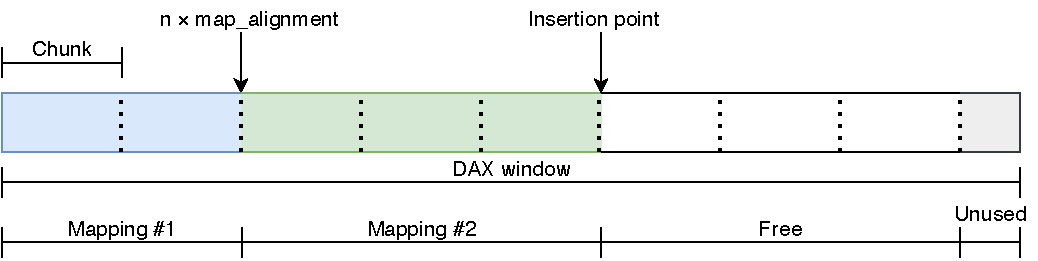
\includegraphics[width=\textwidth]{dax}
    \caption{Ενδεικτική εικόνα του \en{DAX window} υπό τον \en{manager}.}
    \label{fig:dax-overview}
\end{figure}

\begin{figure}
    \begin{minipage}[c][\textheight]{\textwidth}
        \centering
        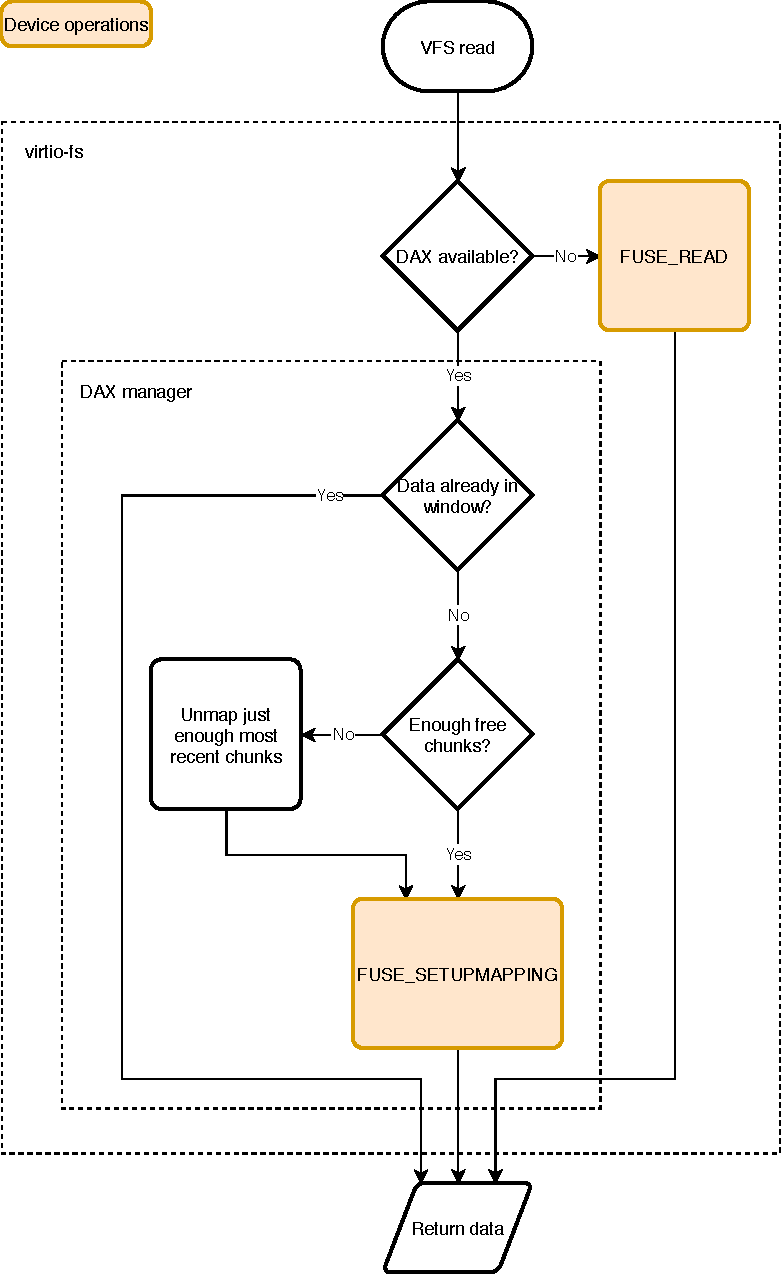
\includegraphics[height=\textheight]{read}
        \caption{Διαδικασία ανάγνωσης από το \viofs{} υπό τον \en{DAX window
            manager}.}
        \label{fig:dax-flowchart}
    \end{minipage}
\end{figure}

\section{\en{Boot} από \viofs{}}

Η προσθήκη υποστήριξης για εκκίνηση (\en{boot}) από το \viofs{} στο \osv{}
είχε δύο συνιστώσες: την κυριότερη που αφορούσε τον πυρήνα του λειτουργικού
συστήματος αλλά και μία βοηθητική που αφορούσε τα εργαλεία αυτοματισμού για τη
δημιουργία και εκτέλεση των εικόνων. Αμφότερες βασίστηκαν σε προηγούμενες
αντίστοιχες επεκτάσεις, μιας και το \osv{} ήδη μπορούσε να χρησιμοποιήσει
είτε το \en{ZFS} είτε το \en{rofs} (και το \en{ramfs} βέβαια, που είναι
ιδιαίτερη περίπτωση) για το κύριο (\en{root}) σύστημα αρχείων του.

Συνοπτικά, τα σημεία που αφορούν το \en{root file system} κατά τον κύκλο ζωής
ενός \osv{} \en{unikernel}, ως είχαν πριν την επέκταση μας είναι:
\begin{enumerate}
    \item Χτίσιμο της εικόνας (κεντρικό σημείο το \en{scripts/build}): σε αυτό
          το στάδιο επιλέγεται από τον χρήστη ο τύπος του συστήματος αρχείων
          και το \en{root file system} δημιουργείται με το περιεχόμενο που
          προκύπτει από την εφαρμογή. Επίσης, εδώ ξεκινά ο καθορισμός της
          εντολής εκκίνησης (\en{command line}) του \en{(uni)kernel}, η οποία
          περιέχει επιλογές για τον ίδιο τον πυρήνα, αλλά και το \en{command
          line} της εφαρμογής που πρόκειται να εκτελεστεί. Αυτή αποθηκεύεται
          σε ένα προσωρινό αρχείο, από όπου την παραλαμβάνει το επόμενο βήμα
          \cite{osv-wiki:osv-components}.
    \item Εκτέλεση της εικόνας (κεντρικό σημείο το \en{scripts/run.py}): εδώ
          προαιρετικά εμπλουτίζεται το \en{command line} με εφήμερες επιλογές,
          για παράδειγμα το επίπεδο λεπτομέρειας (\en{verbosity}) στα μηνύματα
          του πυρήνα. Κατόπιν, το ολοκληρωμένο \en{command line} εγγράφεται στο
          \en{image}, προτού αυτό εκτελεστεί.
    \item Φόρτωση του πυρήνα (κεντρικό σημείο το \en{loader.cc}): μετά από,
          μεταξύ άλλων, την αρχικοποίηση του πυρήνα, των συσκευών και των
          οδηγών, αλλά και το διάβασμα του \en{command line}, το \osv{}
          επιχειρεί να περάσει από το αρχικό, ενσωματωμένο σύστημα αρχείων του
          (\en{ramfs}) στο κύριο σύστημα αρχείων (\en{root file system})
          \cite{osv-wiki:osv-loader}. Η διαδικασία ετούτη συνίσταται στην
          προσάρτηση (\en{mounting}) του συστήματος αρχείων σε κάποιο σημείο του
          υπάρχοντος, αρχικού \en{ramfs}, ακολουθούμενη από το πέρασμα της ρίζας
          (\en{pivoting}) του εικονικού συστήματος αρχείων σε αυτό. Τα τελευταία
          γίνονται απλά, μέσω του εικονικού συστήματος αρχείων, αφού όλα τα
          προαπαιτούμενα για τη χρήση του έχουν ολοκληρωθεί.
\end{enumerate}
% TODO OPT: Diagram with build / run process and flow of relevant options.

Η επιλογή του συστήματος αρχείων που θα χρησιμοποιηθεί ως \en{root} κατά τη
φόρτωση μέχρι πρότινος ήταν δυναμική: γινόταν απόπειρα προσάρτησης από την
πρώτη συσκευή \en{block} αρχικά του \en{rofs} και εάν αυτό αποτύγχανε, του
\en{ZFS}. Εάν αμφότερα αποτύγχαναν, η εκτέλεση συνεχιζόταν με το \en{ramfs}
αρχικό σύστημα αρχείων. Αν και η προηγούμενη διαδικασία θα μπορούσε εύκολα να
επεκταθεί ώστε να συμπεριλάβει το \viofs{}, γινόταν εμφανές ότι βασιζόταν σε
πολλές σιωπηλές υποθέσεις, χωρίς να αφήνει μεγάλο περιθώριο ελέγχου στον χρήστη.
Έτσι αποφασίσαμε να πάμε ένα βήμα παραπέρα, ώστε να δοθεί περισσότερος έλεγχος
επί της διαδικασίας: προσθέσαμε μία επιλογή \texttt{\en{-{}-rootfs}} στη γραμμή
εντολών του πυρήνα (\en{command line option}), η οποία επιτρέπει να καθοριστεί
ρητά ο τύπος του \en{root file system} (ανάμεσα σε \en{ZFS, rofs}, \viofs{} και
\en{ramfs}). Όπως φαίνεται και στο διάγραμμα \ref{fig:rootfs}, αυτή η επιλογή
είναι προαιρετική και εάν δεν έχει καθοριστεί χρησιμοποιείται η παλαιότερη,
δυναμική διαδικασία, για συμβατότητα. Τέλος, κάναμε τις απαραίτητες αλλαγές στη
διαδικασία χτισίματος (\en{scripts/build}) ώστε να θέτει αυτή την επιλογή
ανάλογα με το σύστημα αρχείων που έχει καθορίσει ο χρήστης κατά το χτίσιμο.
Εξάλλου, με αυτόν τον τρόπο έγινε πιο προβλέψιμη και τεκμηριώθηκε καλύτερα η
διαδικασία καθώς και οι διαθέσιμες επιλογές για το \en{root file system}.

\begin{figure}
    \centering
    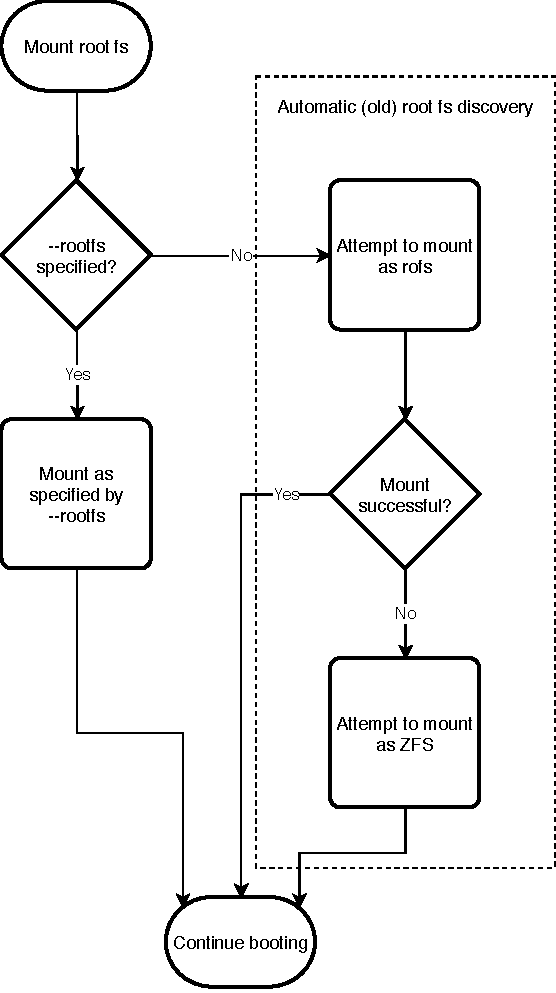
\includegraphics{rootfs}
    \caption{Διαδικασία προσάρτησης του \en{root file system}.}
    \label{fig:rootfs}
\end{figure}

Τέλος, όσον αφορά καθεαυτό το \viofs{}, η χρήση του ως \en{root file system}
δεν ενείχε κάποια αξιοσημείωτη πρόκληση: εάν επιλέγονταν μέσω του
\texttt{\en{-{}-rootfs}}, γινόταν προσάρτηση του από την πρώτη \viofs{} συσκευή
(στο \osv{}, σε αντίθεση με το \linux{}, αυτές εκτίθενται στο \en{devfs},
αριθμημένες σειριακά αντί να αναγνωρίζονται από το \viofs{} \en{tag} τους).
Προκειμένου να συμπληρωθεί αυτόματα με τα κατάλληλα περιεχόμενα για την εκάστοτε
εφαρμογή ένας κατάλογος στον \host{} (ο οποίος στη συνέχεια θα χρησιμοποιηθεί
ως το \viofs{} \en{shared directory}), είναι διαθέσιμες οι παράμετροι
\texttt{\en{export}} και \texttt{\en{export\_dir}} του \en{scripts/build}.
